\subsection{Optimization Methodology}
\begin{frame}
    \frametitle{AHTR Optimization Problem Definitions}
    \begin{block}{Varied Input Parameters}
        \begin{itemize}
            \item TRISO fuel packing fraction fraction distribution 
            \item Total fuel packing fraction 
            \item Coolant channel shape 
        \end{itemize}
    \end{block}
    \begin{block}{AHTR Optimization Objectives}
        \begin{figure}
            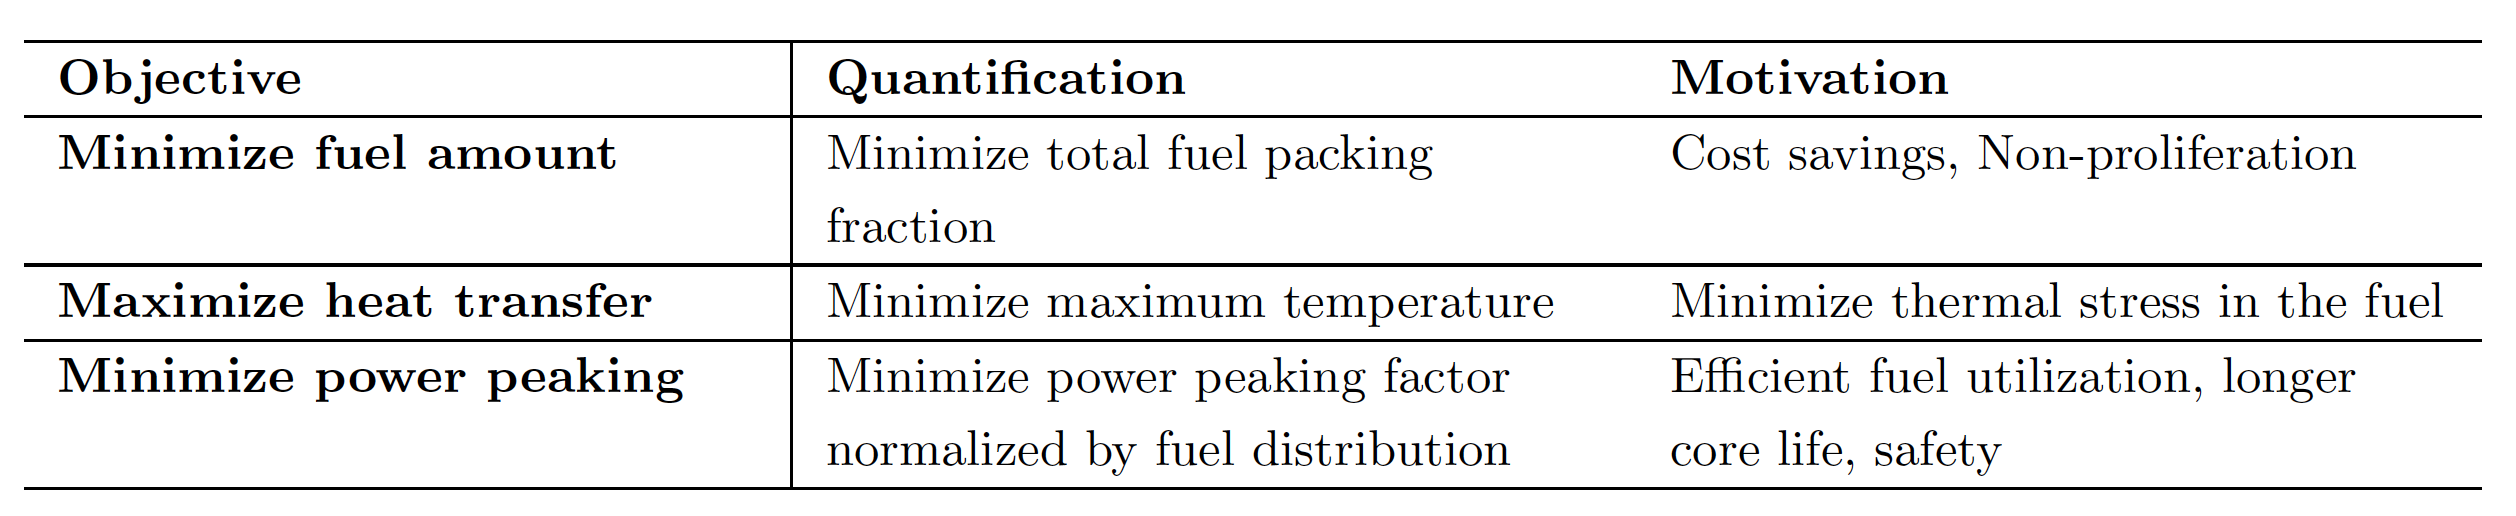
\includegraphics[width=0.9\linewidth]{figures/ahtr-opt-obj.png} 
            \caption{Optimization problem objectives.}
        \end{figure}
    \end{block}
\end{frame}

\begin{frame}
    \frametitle{AHTR Plank Geometry}
    A sine distribution governs TRISO packing fraction distribution: 
    \begin{align}
        \rho_{TRISO}(\vec{x}) &= \left(\textbf{a}\cdot sin(\textbf{b}\cdot x + \textbf{c}) + 2\right) \cdot NF \nonumber
    \end{align}
    \begin{figure}
        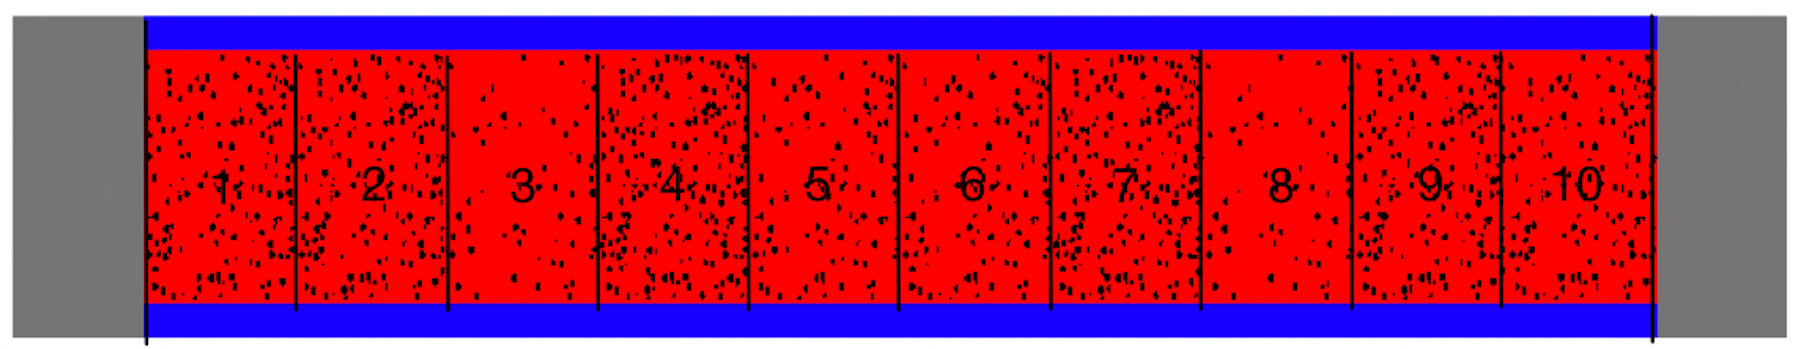
\includegraphics[width=0.9\linewidth]{../docs/figures/straightened_plank.png} 
        \caption{Straightened AHTR Plank with 10 fuel cells with random TRISO packing.}
    \end{figure}
    $r_{top}$ and $r_{bot}$ control coolant channel shape: 
    \begin{figure}
        
\includegraphics[width=\linewidth]{../docs/figures/coolant-channel-shape.png} 
        \caption{AHTR Plank with coolant channel shape variation, $r_{top}$ = 0.2cm and 
        $r_{bot}$ = 0.3cm.}
    \end{figure}
\end{frame}

\begin{frame}
    \frametitle{AHTR One-Third Assembly Geometry}
    Two sine distributions govern TRISO packing fraction distribution: 
    \begin{align}
        \rho_{TRISO}(\vec{x}, \vec{y}) &= \left(\textbf{a}\cdot sin(\textbf{b}\cdot x + \textbf{c}) + 2\right) 
    \cdot \left(\textbf{d}\cdot sin(\textbf{e}\cdot y + \textbf{f}) + 2\right) \cdot NF \nonumber
    \end{align}
    $r_1, r_2, r_3, r_4, r_5$ control coolant channel shape.
    \begin{columns}
        \begin{column}{0.5\textwidth}
            \begin{figure}
                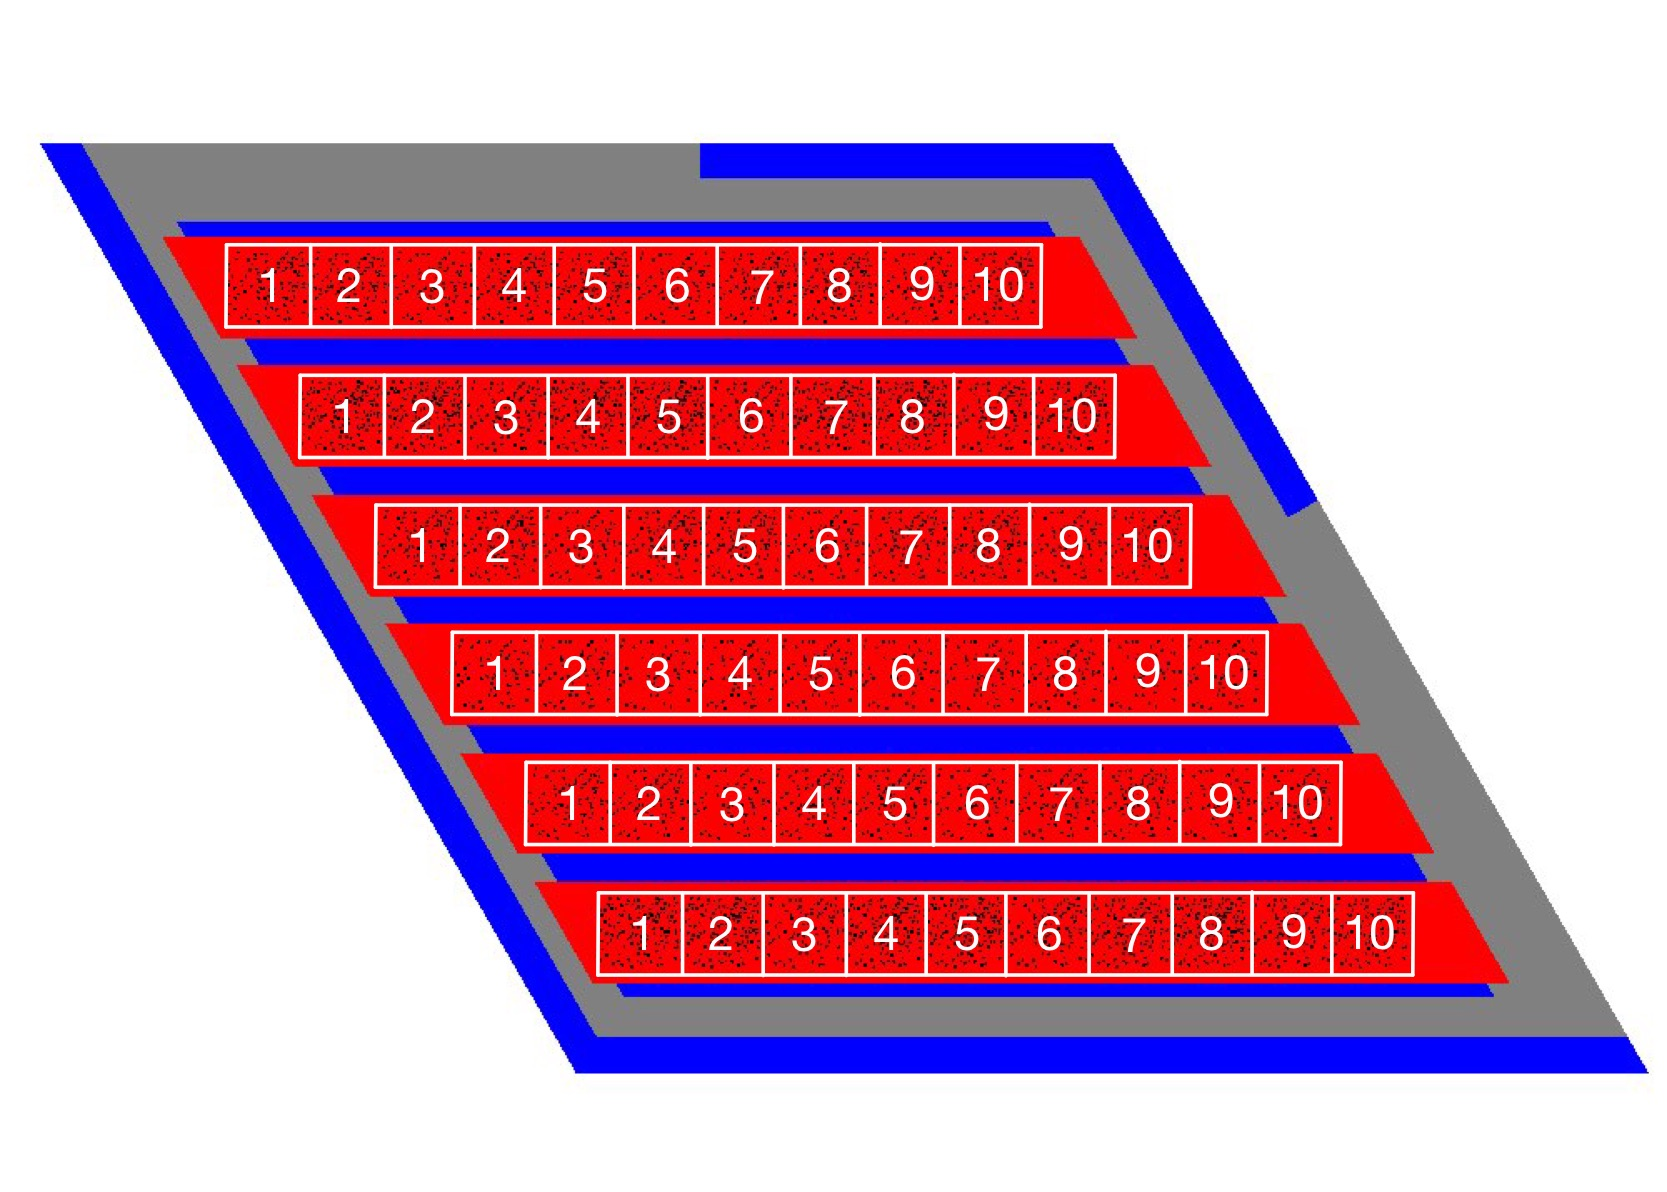
\includegraphics[width=\linewidth]{../docs/figures/ahtr_assembly.png} 
                \caption{AHTR one-third assembly with ten randomly packed fuel cells in 
                each graphite plank.}
            \end{figure}
        \end{column}
        \begin{column}{0.5\textwidth} 
            \begin{figure}
                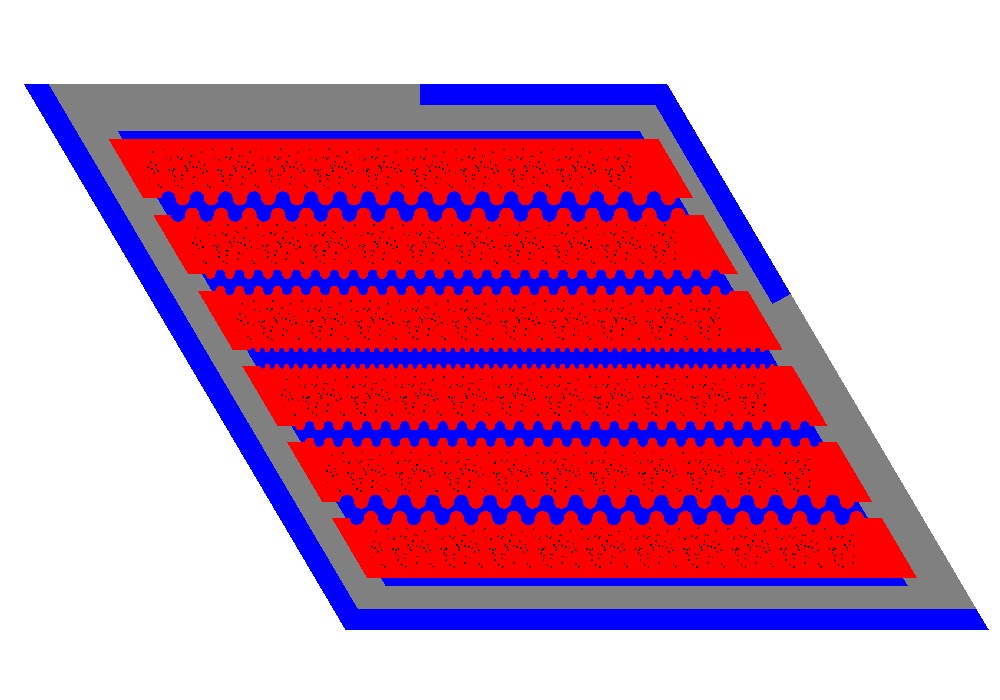
\includegraphics[width=\linewidth]{../docs/figures/coolant-channel-shape-assem.png} 
                \caption{AHTR one-third assembly with coolant channel shape variation, 
                $r_1, r_2, r_3, r_4, r_5$ = 0.3cm, 0.2cm, 0.1cm, 0.2cm, 0.3cm.}
            \end{figure}
        \end{column}
        \end{columns}
\end{frame}

\begin{frame}
    \frametitle{AHTR Modeling Workflow}
    \begin{figure}
        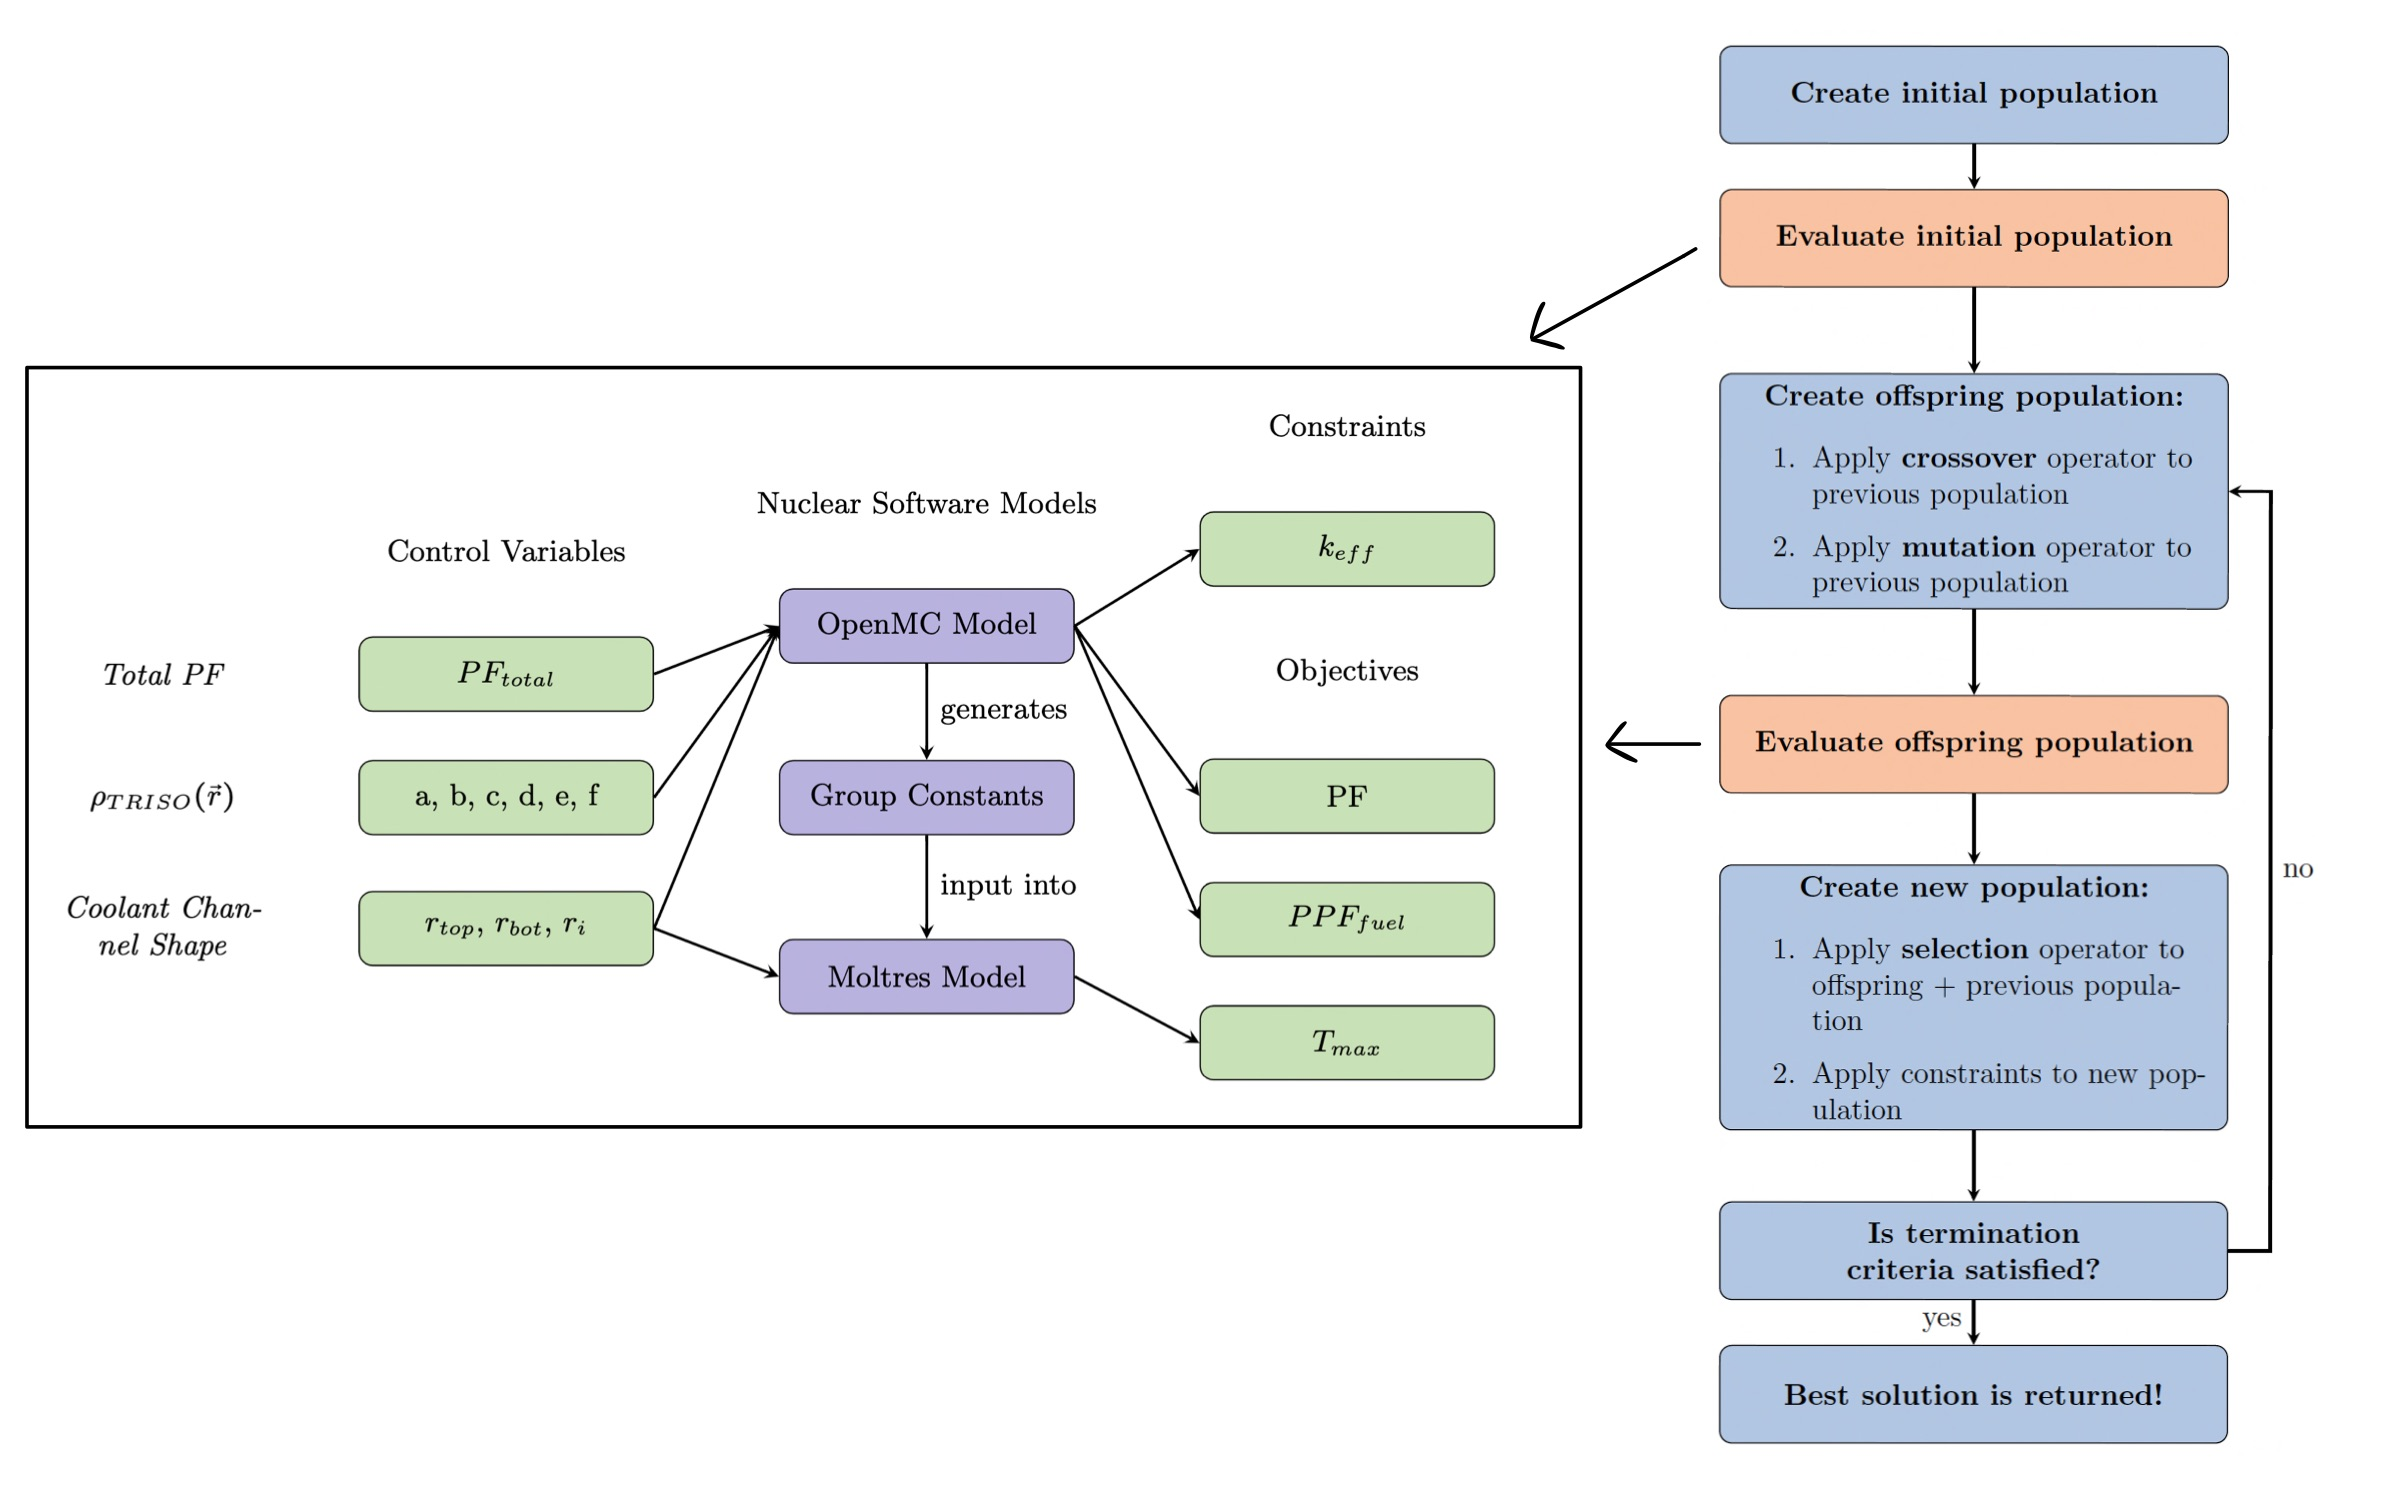
\includegraphics[width=0.95\linewidth]{figures/ahtr-modeling-workflow.png} 
        \caption{AHTR Modeling Workflow.}
    \end{figure}
\end{frame}

\subsection{AHTR Plank Optimization Results}
\frametitle{AHTR Plank Optimization Simulations}
\begin{frame}
\begin{figure}
    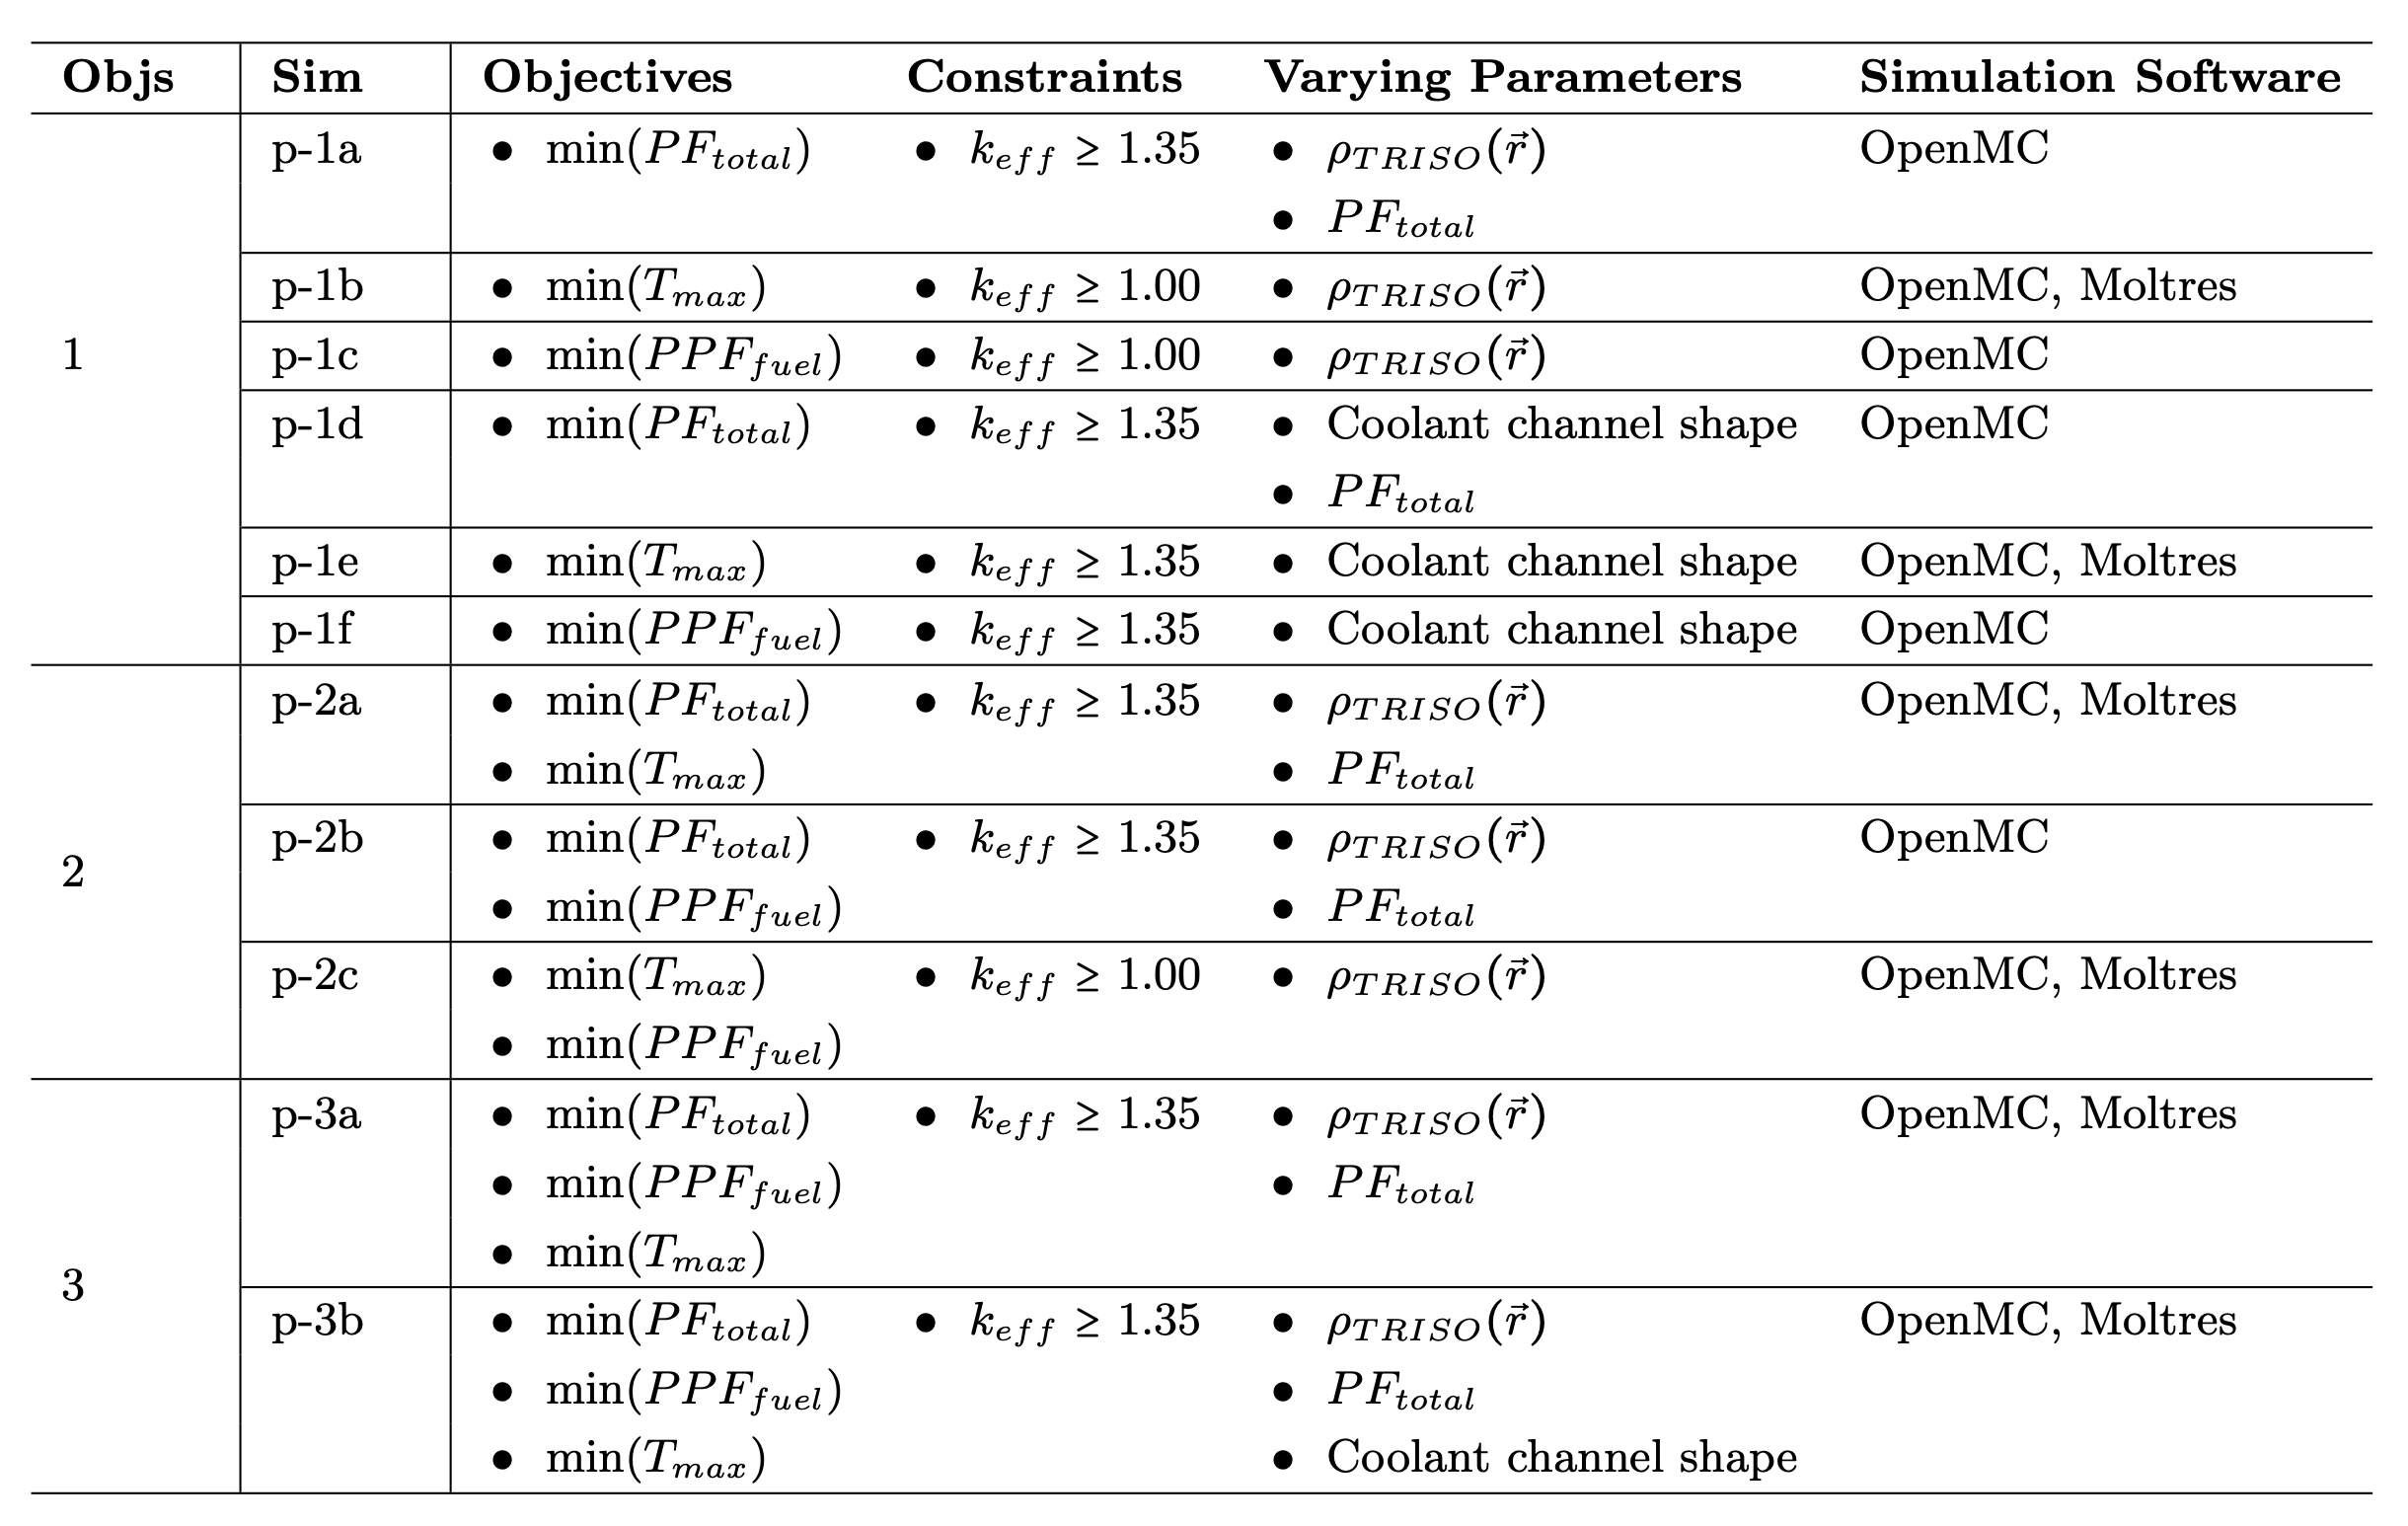
\includegraphics[width=0.95\linewidth]{figures/ahtr-plank-opt-table.png} 
    \caption{simulations.}
\end{figure}
\end{frame}

\subsection{AHTR One-Third Assembly Optimization Results}